\documentclass[12pt]{report}
\usepackage{graphicx}
\usepackage{amsmath}
\begin{document}
	\begin{quote}
		\centering{\textbf{\large Accelerometer and Gyroscope Integration}}
	\end{quote} 
To measure the orientation of the bot we used a GY-80 IMU module.
\begin{figure}[h]
	\centering
	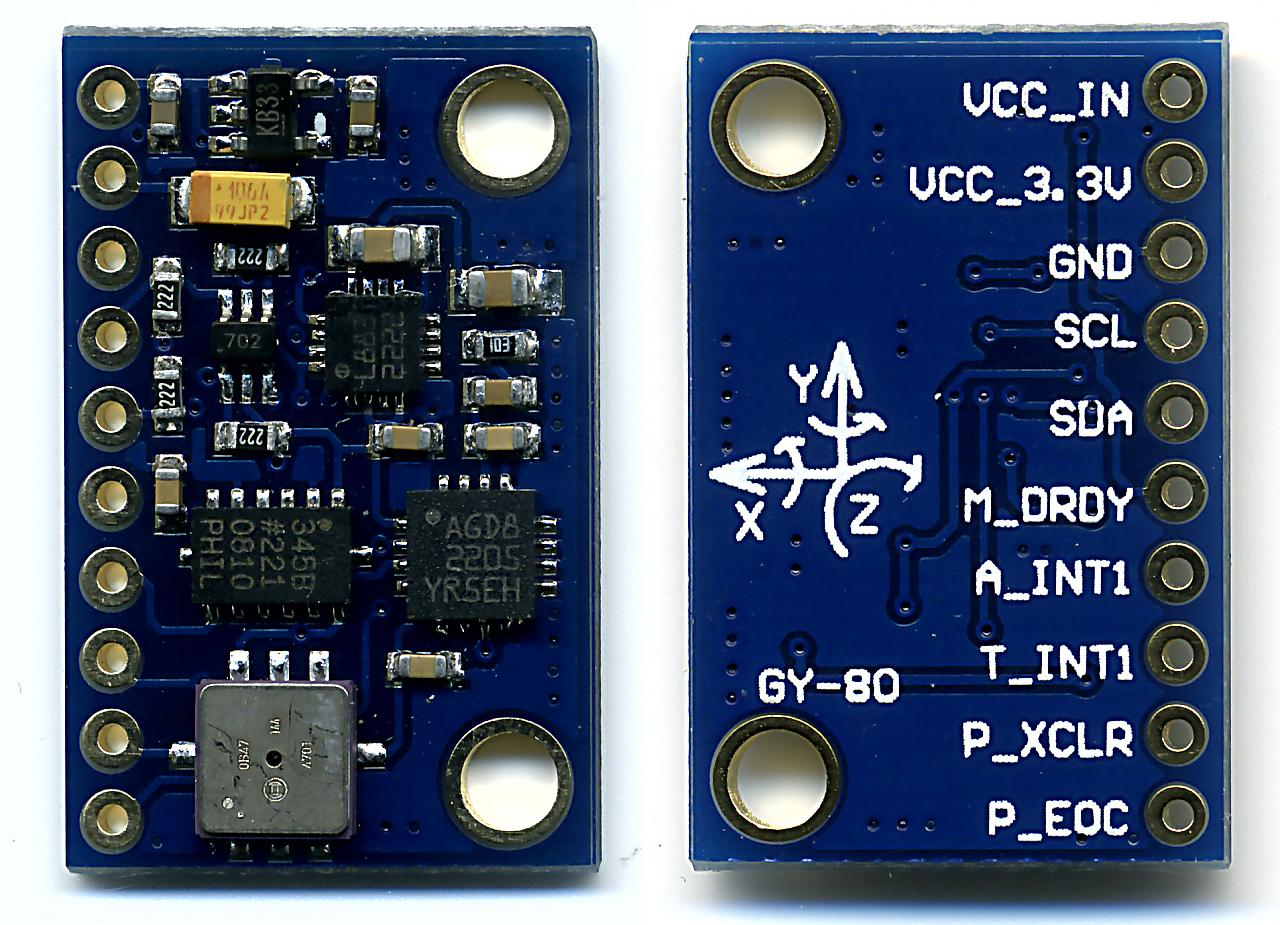
\includegraphics[scale=0.1]{gy80.jpg}
\end{figure} \\
This module includes:-
\begin{itemize}
	\item AGD8 (3-Axis Angular Rate Sensor or Gyroscope)
	\item ADXL345 (3-Axis Digital Accelerometer)
	\item HMC5883L (3-Axis Digital Compass or Magnetometer)
	\item BMP085 (Barometric Pressure Sensor)
\end{itemize} 
We are using only accelerometer and gyroscope sensors with six degree of freedom(DOF).\\
\textbf{Accelerometer:-}It gives the components of acceleration(g) along its three axis.Accelerometers are often used to calculate a tilt angle. They can only do this reliably when they are static and not moving. To get an accurate angle of tilt they are often combined with one or more gyro's and the combination of data is used to calculate the angle.

Digital accelerometers will give us information using a serial protocol like I2C , SPI or USART.We are using I2C protocol to get information from accelerometer.Code for the I2C communication can be found in code documentation part.

We placed accelerometer in such a way that component of g along x-axis is always zero so we have only y and z axis components.So vertical angle of the bot from the z-axis is given by:- \\
\begin{quote}
\centering	$ Angle =\arctan {\frac{y}{z}} $
\end{quote}
Following is the code for calculating angle from ADXL345:-\\ \\ \\ \\
\begin{figure}[h]
	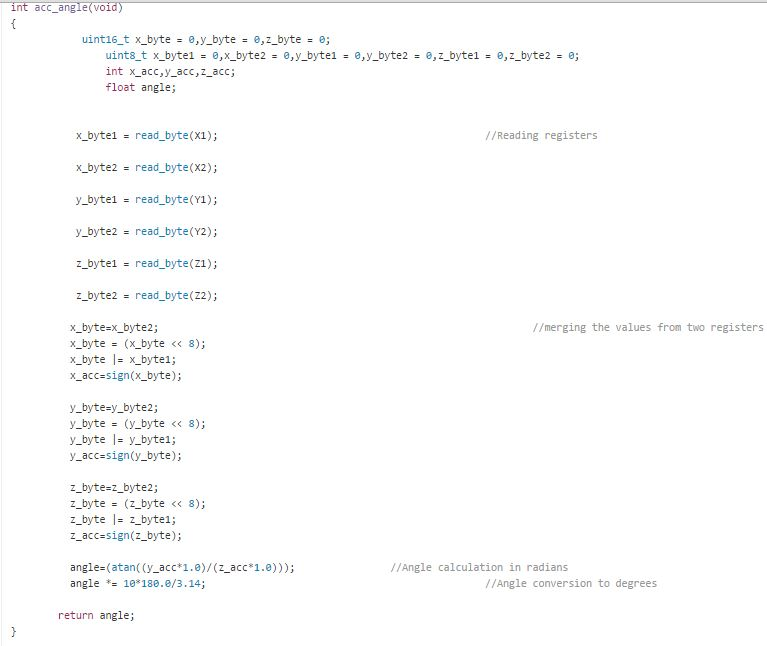
\includegraphics[scale=0.7]{acc.jpg}
\end{figure}\\
\textbf{Accelerometer data is generally more sensitive to the noise.}\\ \\
\textbf{Gyroscope:-}It gives the components of angular
velocity along its three axis.Unlike accelerometers a gyro's output is linear to the rate of rotation measured in degrees per second.Gyro's response is fast so they are good at producing a quick response to a change in angle

Digital accelerometers will give us information using a serial protocol like I2C , SPI or USART.We are using I2C protocol to get information from gyroscope.

We placed gyroscope in such a way that angular velocity in y and z direction is zero,so we have only x direction component. \\

Following is the code for getting output from gyroscope:-
\begin{figure}
	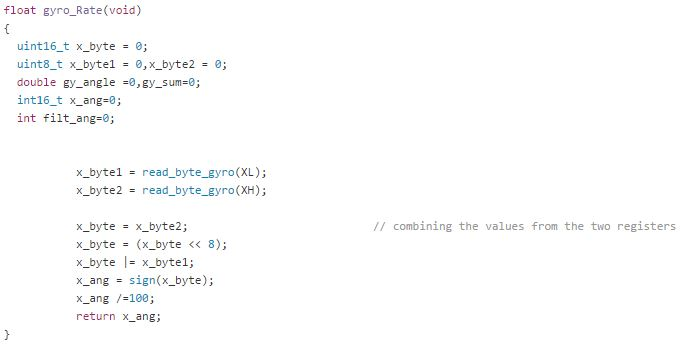
\includegraphics{gyro.jpg}
\end{figure} \\
\textbf{Gyroscope output is less sensitive but gets DRIFTED along with the time.} \\ \\
\textbf{Complimentary filter:-}So we have Gyros which respond quickly, but drift over time, and we have accelerometers which respond slowly but are accurate over time. We can merge these two sensors readings to give use a quick response which is also accurate.

There are two main methods for integrating gyro and accelerometer readings. The Kalman Filter and the Complimentary Filter. Extensive information on each can be found by searching on the internet.The Complimentary filter is much easier to use, tweak and understand. Also it uses much less code, so is the one we will use here.

Here is the code for the complimentary filter. It takes as inputs, the angle calculated from the accelerometer, and the rate of rotation in degrees/second from the gyro.
filterAngle is the calculated angle from the filter
dt is the time period between taking readings in seconds (e.g. dt=0.02 is a reading rate of 50 times per second)
timeConstant is a value which is used to determine how quickly the calculated angle is corrected by the accelerometer value.Play around with these values to get the best response/accuracy required.
Following is the code for complimentary filter:-\\

\begin{figure}[h]
	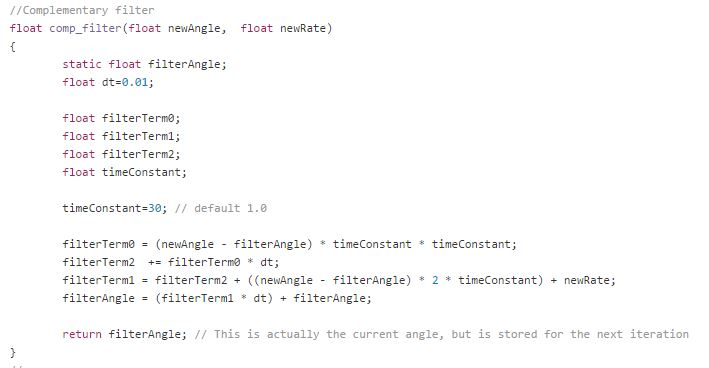
\includegraphics[scale=0.7]{comp_filter.jpg}
\end{figure}

As we were unable to get correct angle from gyroscope so we are using code for complimentary filter which takes input as angle from accelerometer and angular rate from gyroscope.The logic behind this code is that first we are reducing the values from accelerometer by multiplying it with dt,then increasing again its value until it reaches to the final angle,this rate is determined by time constant.By doing so if something noisy data comes in between this short interval complimentary filter avoids it.Angular rate from gyro helps us to reach to the correct final angle as it gives rate of the change of the angle.So we get accurate angle of the bot.
If someone able to get angle from gyroscope then code for complimentary filter will be much easier.\\
Following is the one line code for complimentary filter:-
\begin{quote}
	\centering FiltAngle = HPF * gyroAngle + LPF * accAngle;
\end{quote}
where HPF + LPF =1 \\
Generally HPF = 0.98 and LPF = 0.02 \\
We give more weightage or gain to gyroscope angle and less to the accelerometer angle.
 






\end{document}
